\documentclass[../review_2.tex]{subfiles}
\graphicspath{{\subfix{../img/}}}
\begin{document}

\chapter{Grobentwurf}\thispagestyle{fancy}


Dieses Kapitel behandelt zunächst den Grobentwurf, wie er in der Planungs- und Entwurfsphase des Projekts erarbeitet wurde. Schließlich wird auf dessen Überarbeitung und dazugehörige Diagramme eingegangen. 

\section{Grundlegende Architektur}

In folgendem Unterkapitel werden die grundlegenden Entscheidungen des Entwurfs erklärt und durch die Rahmenbedingungen begründet. Ein intuitiver Einstieg soll schrittweise an das System heranführen über Erklärung des Netzwerkaufbaus, dem grundlegenden Aufbau der Software, dem Kontrollfluss eines Pakets und verwendeter Verfahren.

\subsection{Netzwerkaufbau}
\begin{figure}[h]
    \centering
    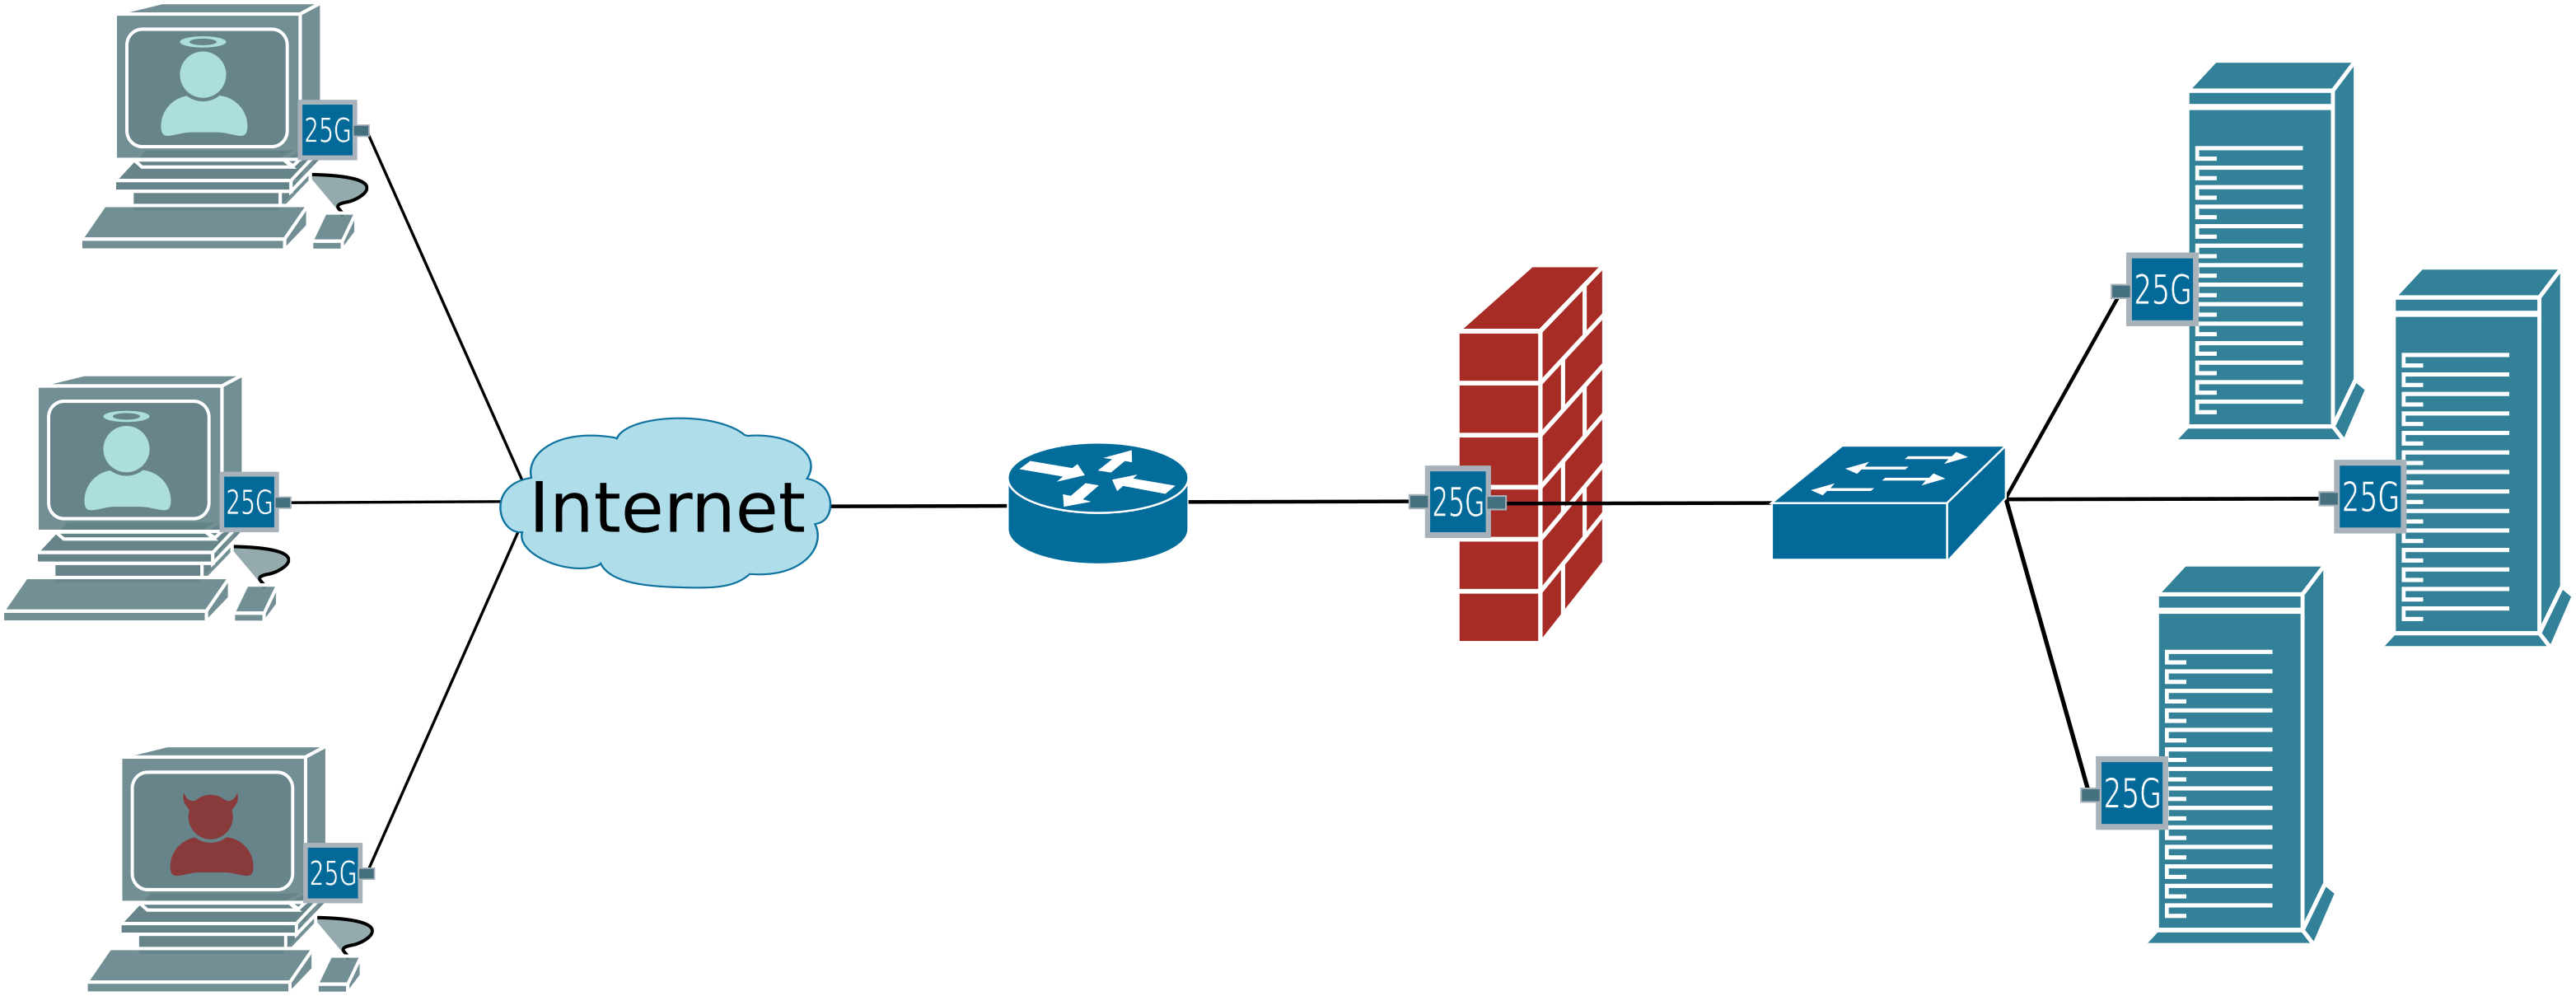
\includegraphics[width=1.0\linewidth]{img/Netzwerkplan-Real}
    \caption{Realaufbau unter Verwendung eines Angreifers}
    \label{fig:netzwerkplan-real}
\end{figure}
Die Abbildung \ref{fig:netzwerkplan-real} zeigen den typischen, zu erwartenden Netzwerkaufbau, welcher in dieser Form im Internet und in der Produktivumgebung vorkommt. Das System untergliedert sich grob in drei Teile. Links in der Abbildung ist jeweils das Internet zu erkennen. In diesem sind unterschiedliche Netzwerke mit jeweils verschiedenen Computern miteinander verbunden. Unter den vielen Computern im Internet, welche für Serversysteme teilweise harmlos sind, befinden sich allerdings auch einige Angreifer. Hier ist ganz klar eine Unterscheidung zwischen dem Angriff eines einzelnen Angreifers, oder einer Menge von einem Angreifer gekapterten und gesteuerten Computer, also eines Botnets, vorzunehmen. 

Wird das Internet, hin zum zu schützenden Netzwerk, verlassen, so wird zuerst ein Router vorgefunden, welcher Aufgaben wie die Network Address Translation vornimmt. Hinter diesem Router befände sich im Produktiveinsatz nun das zu entwickelnde System. Router und zu entwickelndes System sind ebenfalls über eine Verbindung mit ausreichend, in diesem Fall 25Gbit/s, Bandbreite verbunden. Das System selbst agiert als Mittelsmann zwischen Router, also im Allgemeinen dem Internet, und dem internen Netz. Um mehrere Systeme gleichzeitig schützen zu können, aber dennoch die Kosten gering zu halten, ist dem zu entwickelnden System ein Switch nachgeschaltet, mit welchem wiederum alle Endsysteme verbunden sind.

Leider ist durch Begrenzungen im Budget, der Ausstattung der Universität sowie der Unmöglichkeit das Internet in seiner Gesamtheit nachzustellen ein exakter Nachbau des Systems für dieses Projekt nicht möglich. Deswegen musste ein alternativer Aufbau gefunden werden, der allerdings vergleichbare Charakteristika aufweisen muss.

\begin{figure}[h]
    \centering
    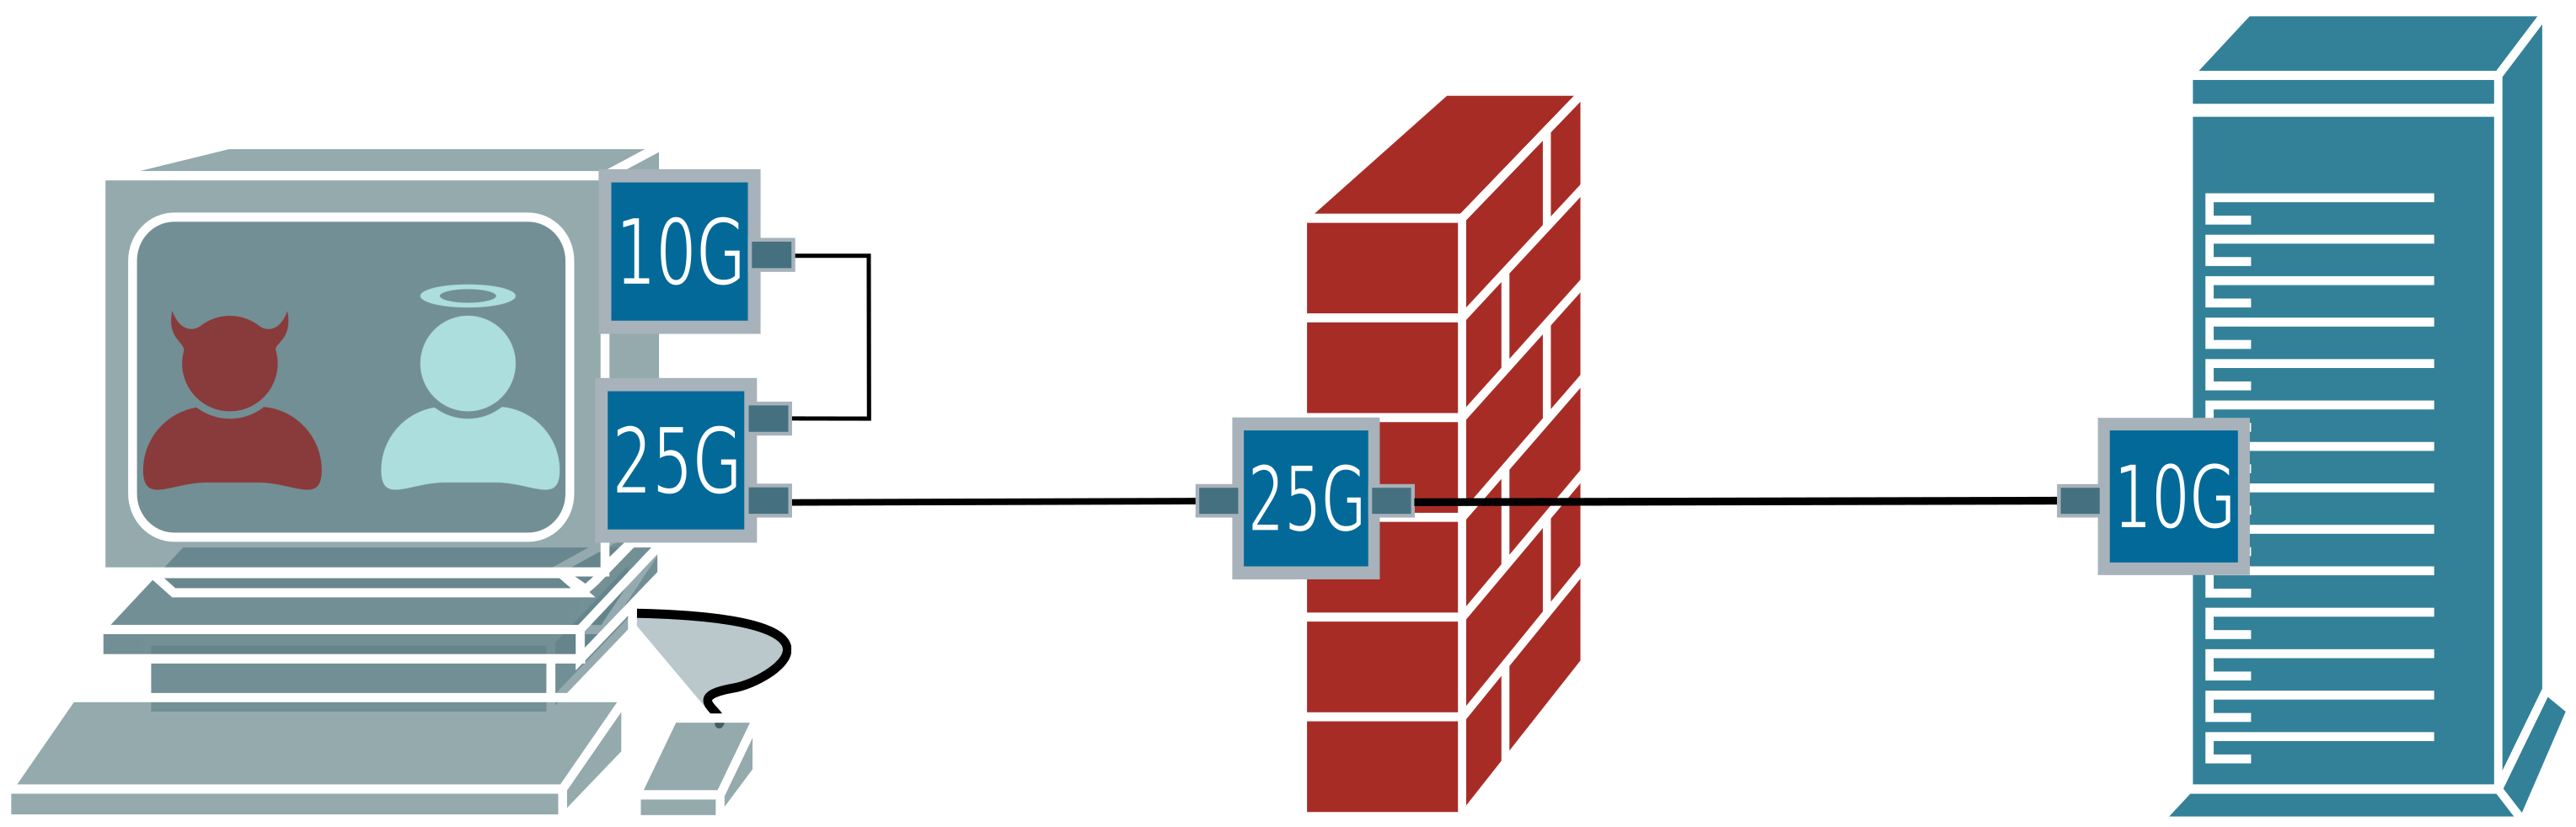
\includegraphics[width=0.7\linewidth]{img/Netwerkplan-Versuch}
    \caption{Versuchsaufbau}
    \label{fig:Versuchsaufbau}
\end{figure}

Der für das Projekt verwendete Versuchsaufbau untergliedert sich ebenfalls in drei Teile. Auch hier beginnt die Darstellung \ref{fig:Versuchsaufbau} ganz links mit dem System, welches Angreifer und legitimen Nutzer in sich vereint. Um die Funktionalität von Angreifer und Nutzer gleichzeitig bereitstellen zu können, setzt der Projektstab, in diesem Fall auf das Installieren zweier Netzwerkkarten, in einem Computer. Eine 10Gbit/s Netzwerkkarte ist mit der Aufgabe betraut, legitimen Verkehr zu erzeugen. Da aufgrund der Hardwarerestriktionen keine direkte Verbindung zur Middlebox aufgebaut werden kann, wird der ausgehende Verkehr dieser Netzwerkkarte in einen Eingang einer zweiten, in demselben System verbauten Netzwerkkarte mit einer maximalen Datenrate von 25Gbit/s eingeführt. Von dieser führt ein 25Gbit/s Link direkt zur Middlebox. Intern wird nun im System, das sich in der Abbildung \ref{fig:Versuchsaufbau} auf der rechten Seite befindet, sowohl legitimer Verkehr erzeugt als auch Angriffsverkehr kreiert, wobei diese beiden Paketströme intern zusammengeführt werden, und über den einzigen Link an die Middlebox gemeinsam übertragen werden. Die Middlebox selbst ist nicht nur mit dem externen Netz verbunden, sondern hat über die selbe Netzwerkkarte auch noch eine Verbindung ins interne Netz. Das gesamte interne Netz wird im Versuchsaufbau durch einen einzelnen, mit nur 10Gbit/s angebundenen Computer realisiert.

Die Entscheidung zur Realisierung in dieser Art fiel, da insbesondere der Fokus darauf liegen soll, ein System zu erschaffen, welches in der Lage ist, mit bis zu 25Gbit/s an Angriffsverkehr und legitimen eingehenden Verkehr zurechtzukommen. Aus diesem Grund ist es ausreichend, eine Verbindung zum internen Netz mit nur 10Gbit/s aufzubauen, da dieses System bei erfolgreicher Abwehr und Abschwächung der Angriffe mit eben diesen maximalen 10Gbit/s an legitimen Verkehr zurecht kommen muss. Ursächlich für die Verwendung der 10Gbit/s Netzwerkkarte im externen Rechner, welcher hierüber den legitimen Verkehr bereitstellen soll, ist, dass der Fokus bei einem solchen Schutzmechanismus natürlich darauf beruht, die Datenrate des Angreifers zu maximieren, um das zu entwickelnde System in ausreichendem Maße belasten und somit Stresstests unterwerfen zu können.


\subsection{Grundlegender Aufbau der Software} \label{section:basic_structure}
Das Grundprinzip der zu entwickelten Software soll sein, Pakete auf einem Port der Netzwerkkarte zu empfangen und diese zu einem anderen Port weiterzuleiten. Zwischen diesen beiden Schritten werden die Pakete untersucht, Daten aus diesen extrahiert und ausgewertet. Im weiteren Verlauf des Programms werden Pakete, welche einem Angriff zugeordnet werden, verworfen, und legtime Pakete zwischen dem interen und externen Netz ausgetauscht. Es bietet sich an, hier ein Pipelinemodell zu verwenden, wobei die einzelnen Softwarekomponenten in Pakete aufgeteilt werden. Im \texttt{ConfigurationManagement} werden die initialen Konfigurationen vorgenommen. Das \texttt{NicManagement} ist eine Abstraktion der Netzwerkkarte und sorgt für das Empfangen und Senden von Paketen. Die \texttt{PacketDissection} extrahiert Daten von eingehenden Paketen. Die \texttt{Inspection} analysiert diese Daten und bestimmt, welche Pakete verworfen werden sollen. Das \texttt{Treatment} behandelt die Pakete nach entsprechenden Protokollen. Um die Abarbeitung dieser Pipeline möglichst effizient zu gestalten, soll diese jeweils von mehreren Threads parallel und möglichst unabhängig voneinander durchschritten werden.

In den folgenden Sektionen wird auf den Kontrollfluss innerhalb des Programms, auf den Einsatz von parallelen Threads und auf die einzelnen Komponenten näher eingegangen.

\subsubsection{Einsatz von parallelen Threads}
Zunächst ist jedoch ein wichtiger Aspekt der Architektur hervorzuheben. Von der Mitigation-Box wird gefordert, eine hohe Paket- und Datenlast verarbeiten zu können. Das Hardwaresystem, auf welchem das zu entwickelnde Programm laufen wird, besitzt eine Multicore-CPU, d.h. das System ist in der Lage, Aufgaben aus unterschiedlichen Threads parallel zu bearbeiten. Dies hat das Potenzial, die Rechengeschwindigkeit zu vervielfachen und so die Bearbeitungszeit insgesamt zu verringern.

Dabei stellt sich die Frage, wozu die Threads im Programm genau zuständig sind. Es wäre zum Beispiel möglich, dass jeder Thread eine Aufgabe übernimmt, d.h. es gäbe einen Thread, der nur Daten analysiert oder aber einen Thread, der nur Paketinformationen extrahiert. Eine solche Aufteilung würde allerdings zu einem hohen Grad an Inter-Thread-Kommunikation führen. Diese ist nicht trivial und kann einen Großteil der verfügbaren Ressourcen benötigen, was den durch die Parallelisierung erzielten Gewinn wieder zunichte machen könnte. Um dieses Risiko zu vermeiden, soll stattdessen jeder Thread die gesamte Pipeline durchlaufen. So ist kaum Inter-Thread-Kommunikation notwendig. Außerdem ist es dann verhältnismäßig einfach, den Entwurf skalierbar zu gestalten: Wenn ein Prozessor mit größerer Anzahl an Kernen verwendet werden würde, könnten mehr Pakete parallel bearbeitet werden, ohne dass die Architektur geändert werden muss.

\subsubsection{Kontrollfluss eines Paketes}

In diesem Abschnitt soll veranschaulicht werden, wie genau die Behandlung eines Paketes vom \texttt{NicManagement} bis zum \texttt{Treatment} erfolgt. Dabei werden die Pakete selbst als Akteure angesehen und nicht deren Klassen. Hinweis: Ein Thread soll später mehrere Pakete auf einmal durch die Pipeline führen. In diesem Diagramm wird zur Übersichtlichkeit jedoch nur der Fluss eines Paketes gezeigt. Dieser lässt sich dann einfach auf eine größere Menge von Paketen anwenden. Ein Aktivitätsdiagramm ist unter Abbildung \ref{fig:control_flow} am Ende der Sektion \ref{section:basic_structure} zu finden.

\begin{figure}[h]
    \centering
    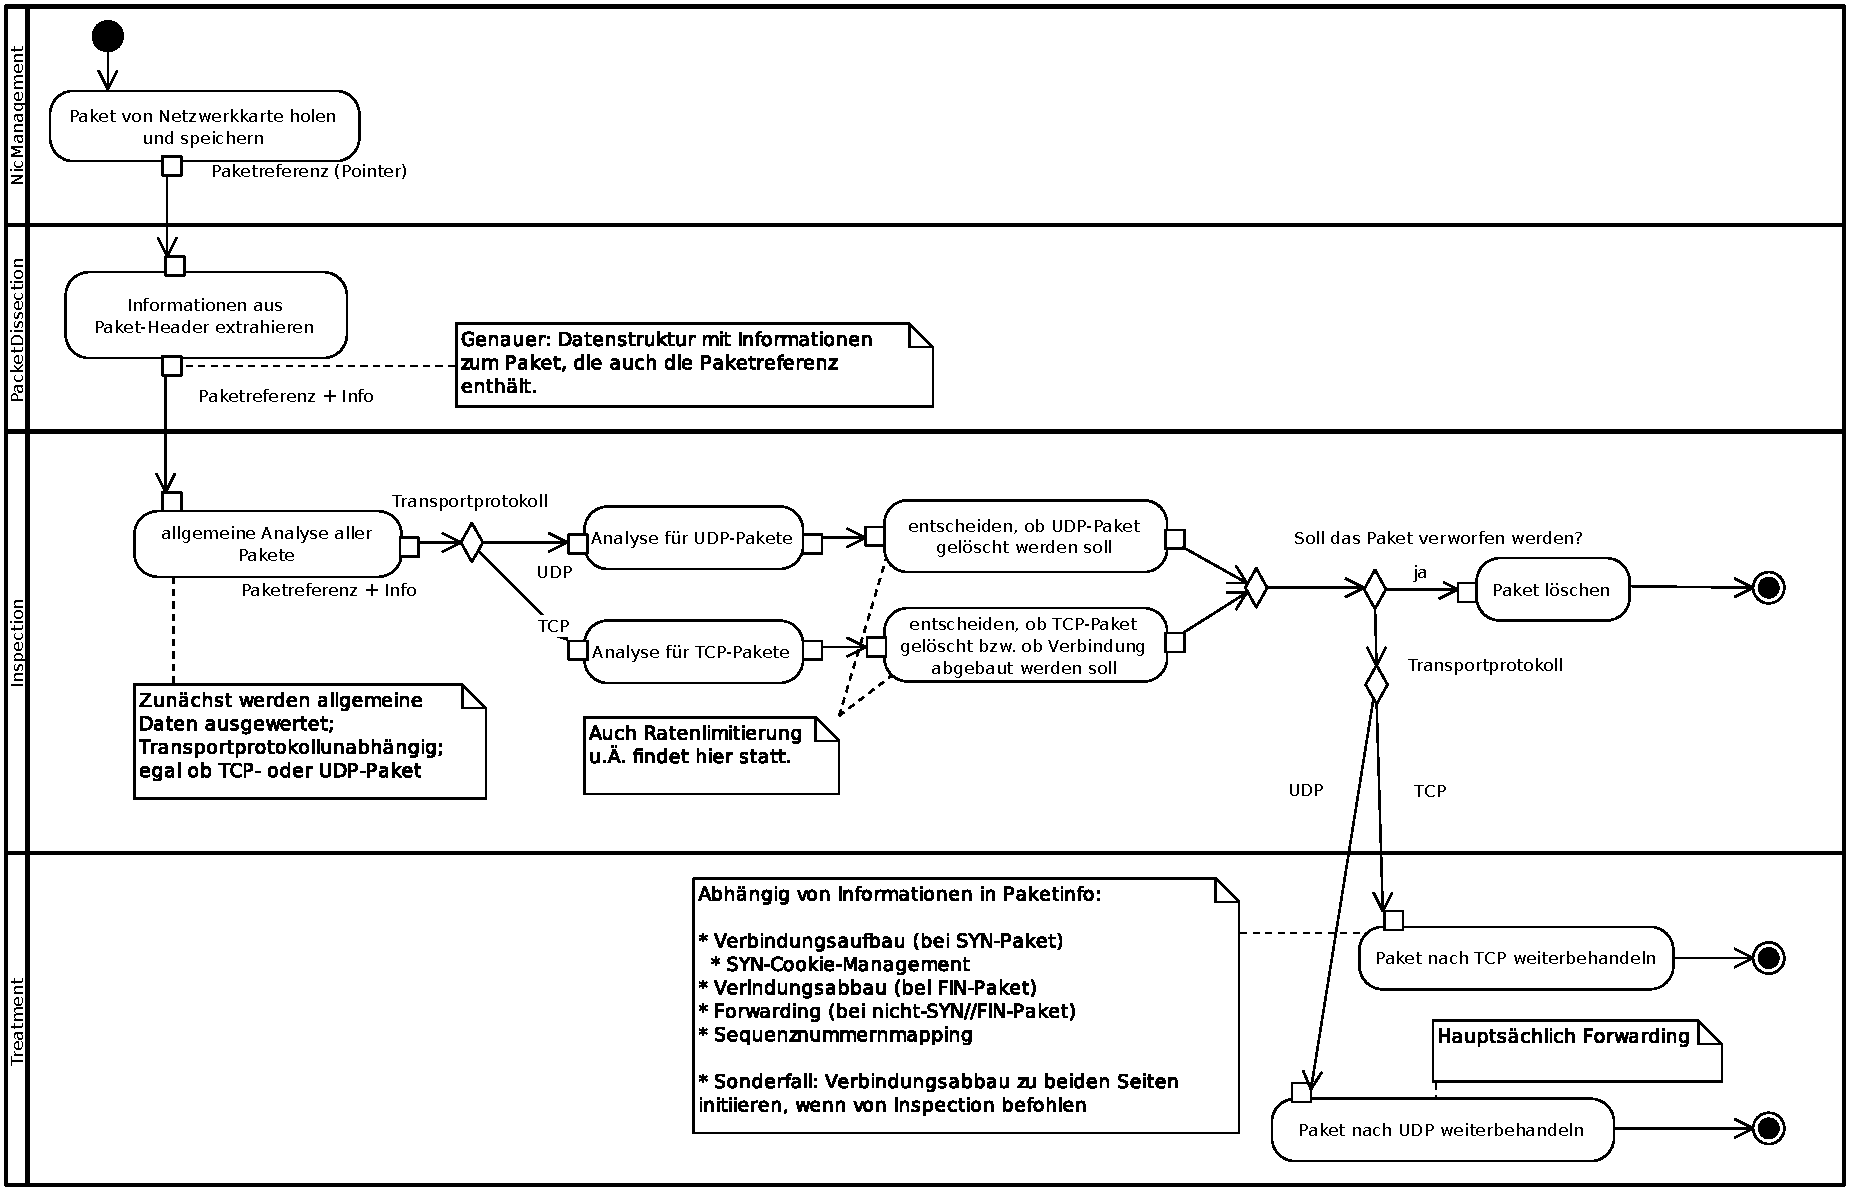
\includegraphics[angle=270, width=0.8\linewidth]{img/activity_control_flow.pdf}
    \caption{Schematische Darstellung des Kontrollflusses}
    \label{fig:control_flow}
\end{figure}

\subsubsection{Verwendung von Receive-Side-Scaling}
Ein weiterer grundlegender Vorteil ergibt sich durch das von der Netzwerkkarte und von DPDK unterstützte Receive Side Scaling (RSS), siehe Abbildung \ref{fig:Receive-Side-Scaling}: Ein auf einem Port eingehendes Paket wird einer von mehreren sogenannten RX-Queues zugeordnet. Eine RX-Queue gehört immer zu genau einem Netzwerkkartenport, ein Port kann mehrere RX-Queues besitzen. Kommen mehrere Pakete bei der Netzwerkkarte an, so ist die Zuordnung von Paketen eines Ports zu seinen RX-Queues gleich verteilt~-- alle RX-Queues sind gleich stark ausgelastet. Diese Zuordnung wird durch eine Hashfunktion umgesetzt, in die Source und Destination Port-Nummer und IP-Adresse einfließen. Das führt dazu, dass Pakete, die auf einem Port ankommen und einer bestimmten Verbindung zugehören, immer wieder zu der selben RX-Queue dieses Ports zugeordnet werden. Mit ,,Port'' im Folgenden entweder der physische Steckplatz einer Netzwerkkarte gemeint oder jener Teil der Netzwerkadresse, die eine Zuordnung zu einem bestimmten Prozess bewirkt. Die Bedeutung erschließt sich aus dem Kontext.

\begin{figure}[H]
    \centering
    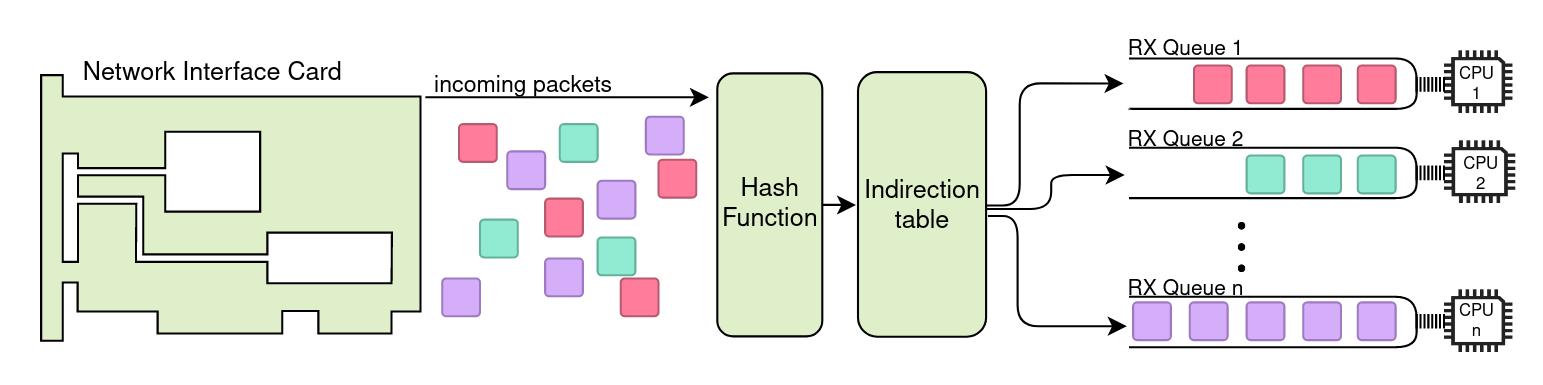
\includegraphics[width=0.95\linewidth]{img/Receive-Side-Scaling.png}
    \caption{Beispielhafte Paketverarbeitung mit Receive Side Scaling}
    \label{fig:Receive-Side-Scaling}
\end{figure}

Ferner besteht die Möglichkeit, Symmetric RSS einzusetzen. Dieser Mechanismus sorgt dafür, dass die Pakete, die auf dem einen Port der Netzwerkkarte ankommen, nach genau der selben Zuordnung auf dessen RX-Queues aufgeteilt werden, wie die auf dem anderen Port ankommenden Pakete auf dessen RX-Queues. Dabei ist die Zuordnung auf dem einen Port ,,symmetrisch'' zu der auf dem anderen Port. Das heißt, wenn bei Port 0 ein Paket mit \texttt{Src-IP: a, Dst-IP: b, Src-Port: x, Dst-Port: y} ankommt, wird es genauso dessen RX-Queues zugeteilt, wie ein Paket mit \texttt{Src-IP: b, Dst-IP: a, Src-Port: y, Dst-Port: x} auf RX-Queues von Port 1. So ergeben sich Paare von RX-Queues, die jeweils immer Pakete von den gleichen Verbindungen beinhalten. Angenommen, die RX-Queues sind mit natürlichen Zahlen benannt und RX-Queue 3 auf Port 0 und RX-Queue 5 auf Port 1 sind ein korrespondierendes RX-Queue-Paar. Wenn nun ein Paket P, zugehörig einer Verbindung V auf RX-Queue 3, Port 0 ankommt, dann weiß man, dass Pakete, die auf Port 1 ankommen und der Verbindung V angehören immer auf RX-Queue 5, Port 1 landen.

Neben RX-Queues existieren auch TX-Queues (Transmit-Queues), die ebenfalls zu einem bestimmten Port gehören. Darin befindliche Pakete werden von der Netzwerkkarte auf den entsprechenden Port geleitet und gesendet. Auf Basis dieses Mechanismus sollen die Threads wie folgt organisiert werden: Einem Thread gehört ein Paar von korrespondierenden RX-Queues (auf verschiedenen Ports) und daneben eine TX-Queue auf dem einen und eine TX-Queue auf dem anderen Port. Das bringt einige Vorteile mit sich: Es müssen zwei Arten von Informationen entlang der Pipeline gespeichert, verarbeitet und gelesen werden: Informationen zu einer Verbindung und Analyseinformationen/Statistiken. Daher ist kaum Inter-Thread-Kommunikation nötig, weil alle Informationen zu einer Verbindung in Datenstrukturen gespeichert werden können, auf die nur genau der bearbeitende Thread Zugriff haben muss. An dieser Stelle soll auch kurz auf eine Besonderheit von DPDK eingegangen werden: Im Linux-Kernel empfängt ein Programm Pakete durch Interrupt-Handling. Gegensätzlich dazu werden bei DPDK alle empfangenen Pakete, die sich derzeit in den RX-Queues der Netzwerkkarte befinden, auf einmal von der Anwendung gepollt. In der zu entwickelnden Software geschieht dieses Polling durch den einzelnen Thread stets zu Beginn eines Pipeline-Durchlaufes.

Im Falle eines Angriffes ist die Seite des Angreifers (entsprechender Port z.B. ,,Port 0'') viel stärker belastet, als die Seite des Servers (z.B. ,,Port 1''). Wegen der gleich verteilten Zuordnung des eingehenden Traffics auf die RX-Queues und weil ein Thread von RX-Queues von beiden Ports regelmäßig Pakete pollt, sind alle Threads gleichmäßig ausgelastet und können die Pakete bearbeiten. Ein günstiger Nebeneffekt bei DDOS-Angriffen ist, dass die Absenderadressen von Angriffspaketen oft sehr unterschiedlich sind. Das begünstigt die gleichmäßige Verteilung von Paketen auf RX-Queues, weil das Tupel aus besagten Adressen der Schlüssel der RSS-Hash-Funktion sind.

\section{Überarbeiteter Grobentwurf}

Die in diesem Abschnitt erläuterten Änderungen wurden im Laufe der Implementierungsphase vorgenommen. Für das bei diesem Softwareprojekt genutzte Vorgehensmodell des Unified Process ist es typisch, dass sich auch während der Implementierung Änderungen am Entwurf ergeben. Für die Teammitglieder ist es besonders aufgrund der geringen Erfahrung bezüglich der Thematik des Projekts unerlässlich, wichtige Verbesserungen direkt vornehmen zu können.

\subsection{Paketdiagramm}

\begin{figure}[H]
    \centering
    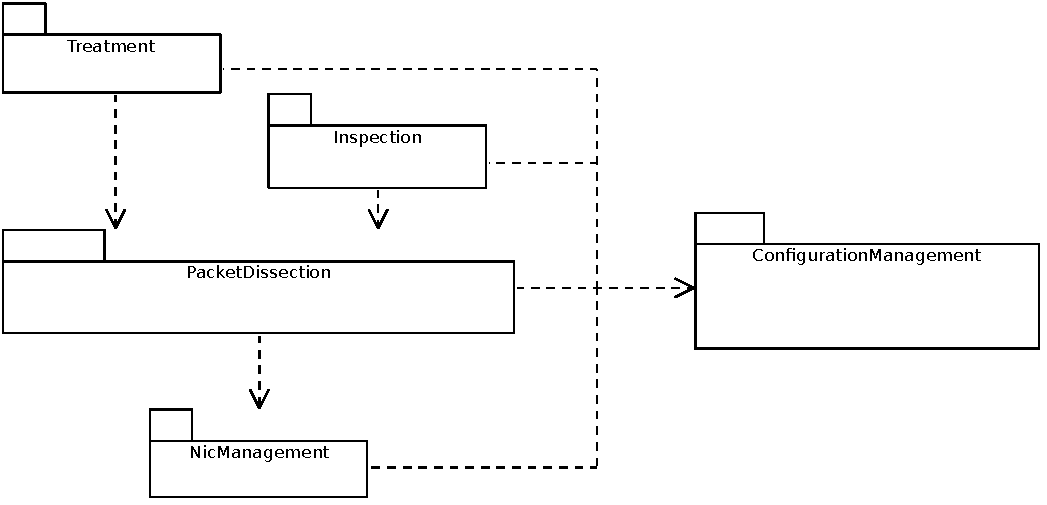
\includegraphics[width=0.82\linewidth]{img/2-grobentwurf/packet_diagram.pdf}
    \caption{Paketdiagramm}
    \label{fig:dospaketdiagramm}
\end{figure}
Grundsätzlich ist es angedacht, wie im Paketdiagramm \ref{fig:dospaketdiagramm} ersichtlich, die zu entwickelnde Software in insgesamt 5 Teile zu untergliedern.

Das \texttt{NicManagement} wird eingesetzt, um die Kommunikation und Verwaltung der Netzwerkkarten und Ports zu ermöglichen, hier finden Operationen wie der Versand und Empfang von Paketen statt. Verwendet wird das \texttt{NicManagement} von der \texttt{PacketDissection}. Diese Komponente beinhaltet Klassen zur Paketrepräsentation für das \texttt{Treatment} und die \texttt{Inspection}. Sie liefert Operationen zum Löschen, Senden, Empfangen und Bearbeiten von Paketen. In der \texttt{PacketDissection} werden auch Informationen aus den einzelnen Headern eines Netzwerkpakets extrahiert.

Die extrahierten Informationen werden von der \texttt{Inspection} verwendet, um sowohl Angriffe erkennen zu können, als auch über den allgemeinen Zustand des Systems in Form von Statistiken Auskunft zu geben. Das \texttt{Treatment}, welches für die Abwehrwehrmaßnahmen der verschiedenen Angriffe zuständig ist, verwendet hierzu die von der \texttt{Inspection} bereitgestellten Ergebnisse und Informationen. Für das Versenden und Verwerfen von Pakten, sowie den Aufbau und das Terminieren von Verbindungen, verwendet das \texttt{Treatment} die \texttt{PacketDissection}, welche die Anweisung an das \texttt{NicManagement} weitergibt.

Sowohl \texttt{Treatment}, als auch \texttt{Inspection} und \texttt{PacketDissection} verwenden das \\ \texttt{ConfigurationManagement}, welches Parameter für die Programmbestandteile in Form von Konfigurationsdateien vorhält. Das \texttt{ConfigurationManagement} bietet die Möglichkeit für den Nutzer, aktiv Einstellungen am System vorzunehmen.


\subsection{NicManagement}
Das \texttt{NicManagement} übernimmt, wie im letzten Review-Dokument erwähnt, das Senden, das Pollen und das Löschen von Paketen. Dieses Paket wurde eingeführt, um bestimmte Funktionen und Initialisierungsschritte vom DPDK zu kapseln. Dabei handelt es sich vor allem um folgende Operationen: \texttt{rte\_eth\_rx\_burst()} und \texttt{rte\_eth\_tx\_burst()} Es hat sich allerdings herausgestellt, dass die Operationen ,,Senden'', ,,Empfangen'' und ,,Löschen'' in der Implementierung sehr wenig Aufwand bereiten. Das Zusammenbauen von Paketen wird von der Komponente \texttt{PacketDissection} übernommen. Der aufwändigere Teil ist die Initialisierung des DPDK, insbesondere die Ermöglichung von Multithreading und die Konfigurierung von symmetric Receive-Side-Scaling. Die dazu notwendigen Schritte werden jedoch von \texttt{Initializer} bzw in der main.cpp-Datei vor dem Starten der einzelnen Threads durchgeführt und sind nicht mehr Teil des \texttt{NicManagements}.

Aus diesem Grund und weil jeder nicht notwendige Funktionsaufruf Rechenzeit kostet, könnte das \texttt{NicManagement} aufgelöst und die bereitgestellten Funktionen an anderer Stelle implementiert werden. Die einzige Klasse, die das \texttt{NicManagement} zum jetzigen Zeitpunkt verwendet, ist die \texttt{PacketContainer}-Klasse in der Komponente \texttt{PacketDissection}. Es wäre möglich, den Inhalt der \texttt{NicManagement}-Aufgaben in diese Klasse zu verschieben.

\begin{figure}[h]
    \centering
    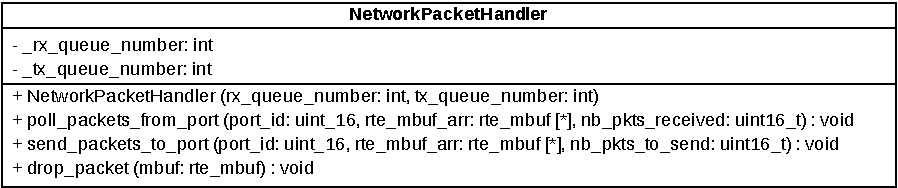
\includegraphics[width=\linewidth]{img/NetworkPacketHandler.pdf}
    \caption{Klassendiagramm: \texttt{NetworkPacketHandler}}
    \label{nph}
\end{figure}

Um ein neues Objekt der Klasse \texttt{NetworkPacketHandler} zu erzeugen, muss der Konstruktor aufgerufen werden. Diesem müssen zwei Parameter übergeben werden (vgl. Abb. \ref{nph}): Zum einen die ID der RX-Queues (\texttt{rx\_queue\_number}), zum anderen die der TX-Queues(\texttt{tx\_queue\_number}).

Für das Verwerfen von Paketen ist die Methode \texttt{drop\_packet()} zuständig. Hierbei muss ein Pointer auf das Paket übergeben werden, das verworfen werden soll.\\
Die Methode  \texttt{poll\_packets\_from\_port()} polllt Pakete von einem spezifischen Port. Dazu werden die ID des Ports, von denen die Pakete gepollt werden sollen, ein Array, auf welches die Pointer der gepollten mbufs geschrieben werden sollen und die Anzahl der Pakete, die in das Array gepollt werden sollen, benötigt.
Ähnliche Parameter werden der Methode \texttt{send\_packets\_to\_port()} übergeben.

\subsection{ConfigurationManagement}
Das Paket \texttt{ConfigurationManagement} kümmert sich um die Initialisierung der Software. Desweiteren werden hier die ablaufenden Threads konfiguriert und verwaltet. Grundlegend ist das Paket in drei Klassen eingeteilt: \texttt{Configurator}, \texttt{Initializer} und \texttt{Thread}. 

\begin{figure}[h]
    \centering
    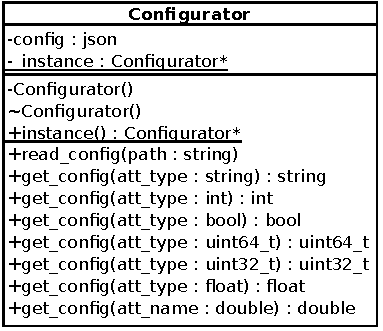
\includegraphics[width=0.4\linewidth]{img/configurator.pdf}
    \caption{Klassendiagramm: \texttt{Configurator}}
    \label{config}
\end{figure}
Die Klasse \texttt{Configurator} bietet eine Schnittstelle zu der Konfigurationsdatei, welche im Projekt liegt und die grundlegenden Einstellungen der Software enthält. An anderer Stelle kann dann über verschiedene Methoden auf Konfigurationsinformationen zugegriffen werden. Abbildung \ref{config} zeigt das Klassendiagramm vom \texttt{Configurator}.

\begin{figure}[h]
    \centering
    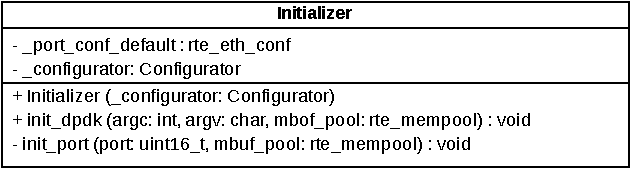
\includegraphics[width=0.7\linewidth]{img/Initializer.pdf}
    \caption{Klassendiagramm: \texttt{Initializer}}
    \label{init}
\end{figure}
Die Klasse \texttt{Initializer} dient dazu die für die Bibliothek DPDK notwendigen Voraussetzungen zu schaffen. Das Klassendiagramm befindet sich in Abb. \ref{init}.

\begin{figure}[h]
    \centering
    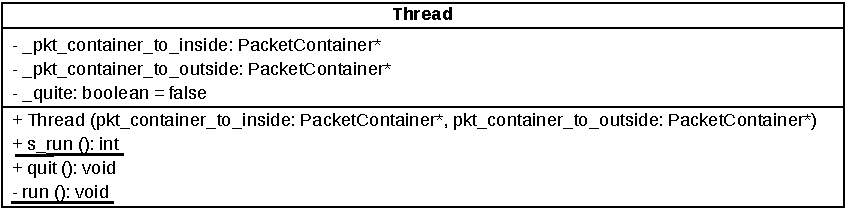
\includegraphics[width=0.85\linewidth]{img/Thread.pdf}
    \caption{Klassendiagramm: \texttt{Thread}}
    \label{thread}
\end{figure}
Die Klasse \texttt{Thread} enthält den Ablaufplan für die Workerthreads des Systems (vgl. Abb. \ref{thread}). 

\subsection{PacketDissection}
Der  Zweck dieses Pakets ist, sämtliche Daten, die \texttt{Analyser} und \texttt{Treatment} für ihre Arbeit brauchen, aus den Paketen zu extrahieren. 

Dafür war geplant, in dieser Komponente die Repräsentation eines Paketes - die Klasse \texttt{PacketInfo} - unterzubringen. Jedes Paket sollte einzeln repräsentiert durch die Pipeline des Programms gereicht werden. Es hat sich herausgestellt, dass dieses Vorgehen ineffizient ist. Näheres dazu ist im Feinentwurfskapitel beschrieben. 

Aus diesem Grund wurde eine neue Klasse namens \texttt{PacketContainer} eingeführt. Diese dient als Repräsentation einer Folge von Paketen, die empfangen wurden. Enthalten sind sowohl die Pointer auf die tatsächlichen Pakete, als auch Metadaten in Form mehrerer Objekte der PacketInfo-Klasse. Im \texttt{PacketContainer} ist es möglich, Pakete zu entnehmen, hinzuzufügen und zu löschen. Weiterhin gibt es jeweils eine Methode zum Pollen neuer Pakete und zum Senden aller vorhandener Pakete. 

Die \texttt{PaketInfo}-Klasse stellt immer noch alle relevanten Header-Informationen eines Paketes zur Verfügung. Allerdings werden Informationen nur noch auf Abruf extrahiert. Hierbei werden für die IP Versionen 4 und 6, sowie die Layer 4 Protokolle TCP, UDP und ICMP unterstützt. Darüber hinaus soll sie auch das verändern einzelner Informationen im Header ermöglichen.

Die letzte Klasse in der \texttt{PacketDissection} ist der namensgebende \texttt{HeaderExtractor}. Seine Aufgabe wandelte sich vom Extrahieren der Informationen zum Vorbereiten des Extrahieren auf Bedarf.

\subsection{Inspection}

Die zuvor globale Auswertung von Angriffen aller Threads durch eine einzige Instanz wurde ersetzt durch eine lokale threadeigene Auswertung. Berechnete Zahlen und Statistiken wie Paketrate und Angriffsrate werden per Interthreadkommunikation nur noch an eine globale Statistikinstanz gesendet. Dadurch können die Threads unabhängig voneinander agieren und reagieren, die Implementation der Methoden ist deutlich einfacher ausgefallen und die Interthreadkommunikation konnte auf ein einwegiges Minimum begrenzt werden, was der Auswertungsgeschwindigkeit jedes Inspection-Threads zugute kommt.

\begin{figure}[h]
    \centering
    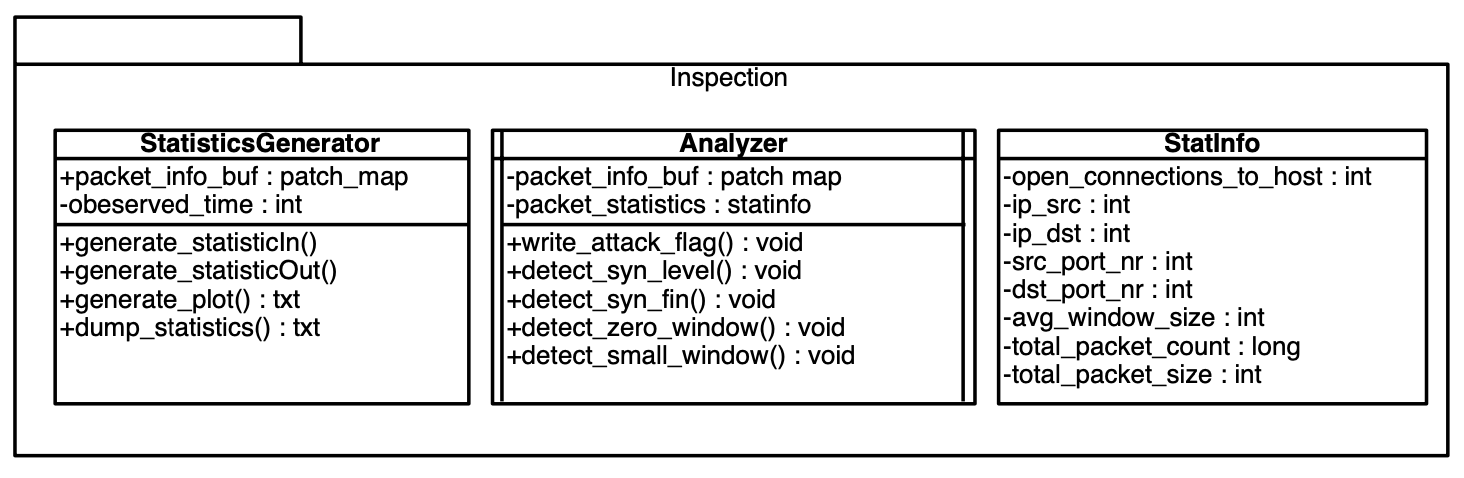
\includegraphics[width=\linewidth]{img/Inspection_old.png}
    \caption{Altes Klassendiagramm der Inspection aus der Implementierungsphase}
    \label{InspectionOld}
\end{figure}

Durch den Einsatz von symetric Receive Side Scaling ist sowohl die Auslastung jeder Inspektion ausgeglichen und zusätzlich werden gleiche Paketströme (selbe Paketquelle und -Empfänger) durch denselben Thread verarbeitet. Dies erleichtert die Erkennung legitimer Pakete, da diese über eine eigene Patchmap für bestimmte Fälle von großteilig illegitimen Verkehr unterscheidbar ist und die Variationen geringer sind.

Die Statistik wird statt durch eine eigene Klasse direkt in der \texttt{Inspection} erstellt und das Ergebnis an eine globale Statistik Instanz gesendet, um diese an den Nutzer auszugeben. Die \texttt{Inspection}-Klasse ist dadurch schlanker und folgt einem linearen Pipelinemodell für Paketverarbeitung.

\begin{figure}[h]
    \centering
    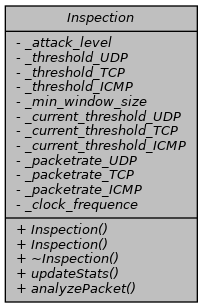
\includegraphics[width=.3\linewidth]{img/Inspection_new.png}
    \caption{Aktuelles Klassendiagramm der Inspection aus der Planungs- und Entwurfsphase}
    \label{AnalyzerNew}
\end{figure}

In Abb. \ref{InspectionOld} und Abb. \ref{AnalyzerNew} lässt sich erkennen, wie sich die \texttt{Inspection} während der Überarbeitung verändert hat.

\subsection{Treatment}

\begin{figure}[h]
    \centering
    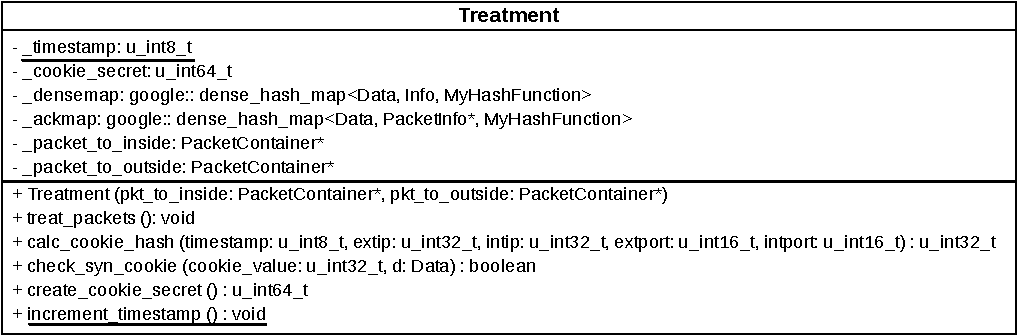
\includegraphics[width=\linewidth]{img/classdia_treatment.pdf}
    \caption{Aktuelles Klassendiagramm des Treatments aus der Implementierungsphase}
    \label{Treatmentclassdia}
\end{figure}

\begin{figure}[h]
    \centering
    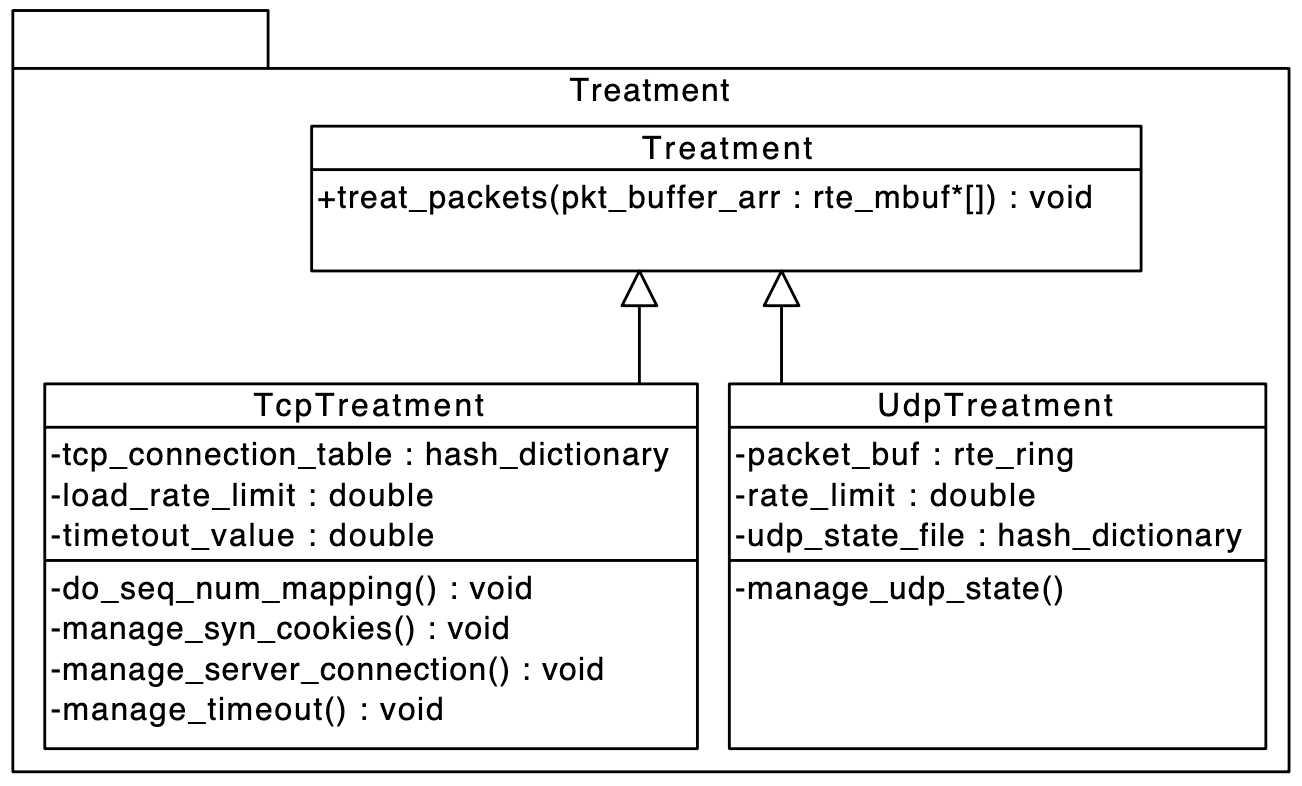
\includegraphics[width=0.7\linewidth]{img/package_Treatment.png}
    \caption{Altes Paket Treatments mit verschiedenen Klassen aus der Planungs- und Entwurfsphase}
    \label{Treatmentclassdia2}
\end{figure}

Abbildung \ref{Treatmentclassdia} zeigt das während der Implementierungsphase überarbeitete Klassendiagramm. Auf den ersten Blick unterscheidet sich dieses stark vom Grobentwurf des \texttt{Treatments} aus der Planungs- und Entwurfsphase (vgl. Abb. \ref{Treatmentclassdia2}).

Das \texttt{Treatment} hat fortan die Aufgabe, die Implementierung von TCP-SYN-Cookies sowie die Realisierung eines TCP-Proxies zu übernehmen. Zur Realisierung des TCP-Proxies gehört insbesondere die Sequenznummernanpassung zwischen internen und externen Verbindungen.

Es fällt auf, dass keine Vererbung mehr verwendet wird. Das heißt, dass nicht mehr zwischen \texttt{TcpTreatment} und \texttt{UdpTreatment} unterschieden wird. Der Grund hierfür ist die Auslagerung des UDP-Treatments in den \texttt{Analyzer} (Paket \texttt{Inspection}). Es wird allerdings nicht nur das UDP-Treatment ausgelagert, sondern auch die Behandlung der SYN-FIN-Attacke sowie des TCP-Small- und Zero-Window-Angriffs. Dies ist darin begründet, dass bereits im \texttt{Analyzer} alle hierzu benötigten Informationen und Funktionalitäten bereitstehen. Dies führt letztlich dazu, dass Funktionsaufrufe oder function calls reduziert werden, welches es dem Programm ermöglicht, insgesamt eine bessere Performanz aufzuweisen.
Durch den Wegfall der Klasse \texttt{UdpTreatment} entfällt die Notwendigkeit der Vererbung und die gesamte Implementierung des Treatments kann in einer einzigen Klasse erfolgen.

Das ursprüngliche Attribut \texttt{tcp\_connection\_table} wurde umbenannt in \texttt{\_densemap}. Der Unterstrich vor dem Variablennamen zeigt, dass es sich um eine Member-Variable handelt. Durch die Umbennenung wird  deutlich, dass es sich um eine Google-Densemap handelt und nicht um eine beliebige Map. Die Densemap untergliedert sich in drei Teile: \texttt{Data} ist der Key (vgl. Abb. \ref{data}), die Info ist die Nutzlast (vgl. Abb. \ref{info})  und der Hashwert aus \texttt{Data} ergibt die Position in der Map (vgl. Abb. \ref{MyHashFunction}).
Hinzu kommt zusätzlich die \texttt{\_ackmap}, bei der es sich ebenfalls um eine Densemap handelt. Die ACK-Map hat zur Aufgabe, diejenigen Pakete zwischenzuspeichern, welche im letzten ACK des externen Verbindungsaufbaus am System ankommen und nach erfolgreichem Verbindungaufbau mit dem internen System an ebendieses weitergeleitet werden müssen.
Der Wegfall von \texttt{load\_rate\_limit} und \texttt{timeout\_value} ist ähnlich wie beim \texttt{UdpTreatment} durch die Auslagerung in den \texttt{Analyzer} zu begründen.
Die Variable \texttt{\_timestamp}, die in der Implementierungsphase hinzugekommen ist, wird benötigt, um das Alter der ACKs, welche als Reaktion auf ein SYN-ACK erhalten werden, zu bestimmen.
Das \texttt{\_cookie\_secret} wird im SYN-Cookie verwendet, um es einem potentiellen Angreifer schwieriger zu machen, eine illegitime Verbindung zum System aufzubauen, indem den Cookies ein weiterer schwieriger zu erratender Wert hinzugefügt wird.
Bei den Variablen \texttt{\_packet\_to\_inside} und \texttt{\_packet\_to\_outside} handelt es sich um Pointer zu \texttt{PacketContainern}. Diese speichern die dem Treatment im Konstruktor übergebenen \texttt{PacketContainer}-Pointer für den weiteren internen Gebrauch.

Um ein Objekt der Klasse \texttt{Treatment} zu erzeugen, muss der Konstruktor aufgerufen werden und die beiden Parameter \texttt{pkt\_to\_inside} und \texttt{pkt\_to\_outside} vom Typ \texttt{PacketContainer*} übergeben werden.

Die Sequenznummernzuordnung, die ursprünglich in der Methode \texttt{do\_seq\_num\_mapping()} vorgenommen werden sollte, ist nun Teil der Methode \texttt{treat\_packets()}, welche allumfassend für das gesamte Verbindungsmanagement des TCP-Verkehrs zuständig ist.
Der Inhalt der Methode \texttt{manage\_syn\_cookies()} wurde mit der Überarbeitung auf verschiedene Methoden aufgeteilt: Der Hash-Wert des TCP-SYN-Cookies wird in der Methode \texttt{calc\_cookie\_hash()} berechnet. Das dazu benötigte Cookie-Secret ist der globale Wert \texttt{\_cookie\_secret}, der durch den Rückgabewert der Methode \texttt{create\_cookie\_secret()} initialisiert wird. Dieser Wert ändert sich während des Ablaufs des Programms nicht. \texttt{Check\_syn\_cookie()} vergleicht den Cookie eines ankommenden, zum Verbindungsaufbau gehörenden ACKs mit dem für diese Verbindung erwarteten Wert. Dazu wird der Methode unter anderem ein Pointer auf ein \texttt{Data}-Objekt übergeben. Der Aufbau der Klasse \texttt{Data} ist in Abb. \ref{data} genauer dargestellt.
Die Methode \texttt{manage\_timeout()} wurde aus oben genannten Effizienzgründen und der Zugehörigkeit zur Behandlung der Sockstress-Attacken (TCP-Small- bzw. TCP-Zero-Window) ebenfalls in den \texttt{Analyzer} verschoben. 
Die Methode \texttt{manage\_server\_connection()} wurde mit der Methode \texttt{treat\_packets()} konsolidiert, um auch hier Funktionsaufrufe einzusparen.
\begin{figure}[h]
    \centering
    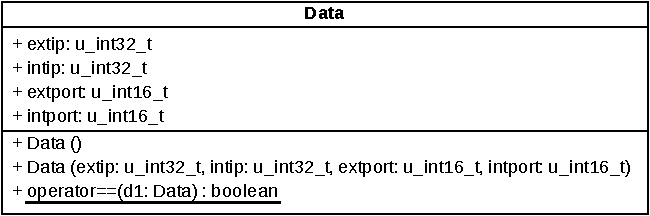
\includegraphics[width=0.7\linewidth]{img/Data.pdf}
    \caption{Klassendiagramm: \texttt{Data}}
    \label{data}
\end{figure}

\begin{figure}[h]
    \centering
    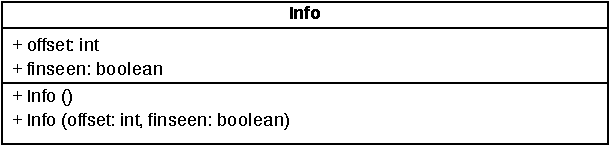
\includegraphics[width=0.7\linewidth]{img/Info.pdf}
    \caption{Klassendiagramm: \texttt{Info}}
    \label{info}
\end{figure}

\begin{figure}[h]
    \centering
    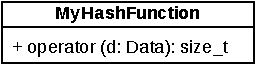
\includegraphics[width=0.3\linewidth]{img/MyHashFunction.pdf}
    \caption{Klassendiagramm: \texttt{MyHashFunction}}
    \label{MyHashFunction}
\end{figure}

\end{document}
